\section{Тестирование}
\label{sec:testing}



\begin{table}[ht]
	\caption{Тест-кейс запуска сервера}
	\label{table:testing:func:test1}
	\centering
	  \begin{tabular}{| >{\raggedright}m{0.4\textwidth} 
					  | >{\raggedright}m{0.3\textwidth} 
					  | >{\raggedright\arraybackslash}m{0.2\textwidth}|}
	  \hline Тест & Ожидаемый результат  & Результат \\
	  \hline \textbf{Старт сервера} \\ 1. Запустить сервер с заданными параметрами командной строки & 1. Появление консольного окна \\ 2. Сообщение о старте сервера & Успех (Рисунок \ref*{sec:testing:func:start})\\
	  \hline
	  \end{tabular}
\end{table}

\begin{figure}[ht]
	\centering
	  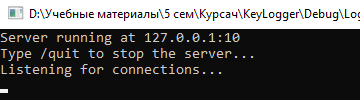
\includegraphics[scale=1]{attachments/serverstart.png}  
	  \caption{ Фрагмент консольного окна сервера }
	  \label{sec:testing:func:start}
\end{figure}

\begin{table}[ht]
	\caption{Тест-кейс обработки запроса клиента на соединение}
	\label{table:testing:func:test2}
	\centering
	  \begin{tabular}{| >{\raggedright}m{0.4\textwidth} 
					  | >{\raggedright}m{0.3\textwidth} 
					  | >{\raggedright\arraybackslash}m{0.2\textwidth}|}
	  \hline Тест & Ожидаемый результат  & Результат \\
	  \hline \textbf{Обработка запроса клиента на соединение} \\ 1. Ожидать входящие соединения & 1. Сообщение о подключенном клиенте и его id & Успех (Рисунок \ref*{sec:testing:func:clientconnect})\\
	  \hline
	  \end{tabular}
\end{table}

\begin{figure}[!htb]
	\centering
	  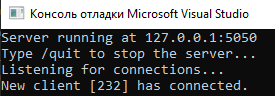
\includegraphics[scale=1]{attachments/clientconnect.png}  
	  \caption{ Фрагмент консольного окна сервера }
	  \label{sec:testing:func:clientconnect}
\end{figure}

\begin{table}[ht]
	\caption{Тест-кейс приема логов нажатых клавиш от клиента}
	\label{table:testing:func:test3}
	\centering
	  \begin{tabular}{| >{\raggedright}m{0.4\textwidth} 
					  | >{\raggedright}m{0.3\textwidth} 
					  | >{\raggedright\arraybackslash}m{0.2\textwidth}|}
	  \hline Тест & Ожидаемый результат  & Результат \\
	  \hline \textbf{Прием логов нажатых клавиш от клиента} \\ 1. Ожидать отправки логов клиентом & 1. Сообщение о получении логов от клиента и его id \\ 2. Файл, содержащий полученные логи & Успех (Рисунки \ref*{sec:testing:func:clientSent}, \ref*{sec:testing:func:logFile})\\
	  \hline
	  \end{tabular}
\end{table}

\begin{figure}[ht]
	\centering
	  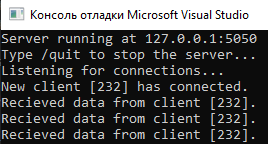
\includegraphics[scale=1]{attachments/clientSent.png}  
	  \caption{ Фрагмент консольного окна сервера }
	  \label{sec:testing:func:clientSent}
\end{figure}

\begin{figure}[ht]
	\centering
	  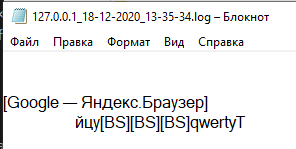
\includegraphics[scale=1]{attachments/logFile.png}  
	  \caption{ Фрагмент лога, записанного на диск }
	  \label{sec:testing:func:logFile}
\end{figure}

\begin{table}[ht]
	\caption{Тест-кейс скрытия папки с программой}
	\label{table:testing:func:test4}
	\centering
	  \begin{tabular}{| >{\raggedright}m{0.4\textwidth} 
					  | >{\raggedright}m{0.3\textwidth} 
					  | >{\raggedright\arraybackslash}m{0.2\textwidth}|}
	  \hline Тест & Ожидаемый результат  & Результат \\
	  \hline \textbf{Скрытие папки с программой} \\ 1. Запустить программное средство отслеживания клавиатурного ввода & 1. Атрибуты папки с исполняемым файлом содержат атрибут Скрытый & Успех (Рисунок \ref*{sec:testing:func:folderProps})\\
	  \hline
	  \end{tabular}
\end{table}

\clearpage

\begin{figure}[ht]
	\centering
	  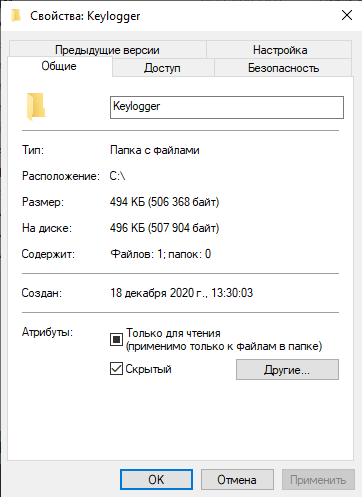
\includegraphics[scale=0.9]{attachments/hiddenFolder.png}  
	  \caption{ Окно свойств папки исполняемого файла}
	  \label{sec:testing:func:folderProps}
\end{figure}

\begin{table}[ht]
	\caption{Тест-кейс добавления программы в автозагрузку}
	\label{table:testing:func:test5}
	\centering
	  \begin{tabular}{| >{\raggedright}m{0.4\textwidth} 
					  | >{\raggedright}m{0.3\textwidth} 
					  | >{\raggedright\arraybackslash}m{0.2\textwidth}|}
	  \hline Тест & Ожидаемый результат  & Результат \\
	  \hline \textbf{Добавление программы в автозагрузку} \\ 1. Запустить программное средство отслеживания клавиатурного ввода & 1. Файл реестра, отвечающий за автозапуск будет содержать ключ, сгенерированный программой & Успех (Рисунок \ref*{sec:testing:func:autorun})\\
	  \hline
	  \end{tabular}
\end{table}

\begin{figure}[!hb]
	\centering
	  
\includegraphics[scale=1]{attachments/autorun.png}  
	  \caption{ Фрагмент реестра }
	  \label{sec:testing:func:autorun}
\end{figure}

\begin{table}[htb]
	\caption{Тест-кейс запрета удаления папки с программой}
	\label{table:testing:func:test6}
	\centering
	  \begin{tabular}{| >{\raggedright}m{0.4\textwidth} 
					  | >{\raggedright}m{0.3\textwidth} 
					  | >{\raggedright\arraybackslash}m{0.2\textwidth}|}
	  \hline Тест & Ожидаемый результат  & Результат \\
	  \hline \textbf{Запрет удаления папки с программой} \\ 1. Запустить программное средство отслеживания клавиатурного ввода & 1. Ошибка, при попытке удаления папки & Успех (Рисунок \ref*{sec:testing:func:deleteerror})\\
	  \hline
	  \end{tabular}
\end{table}

\begin{figure}[htb]
	\centering
	  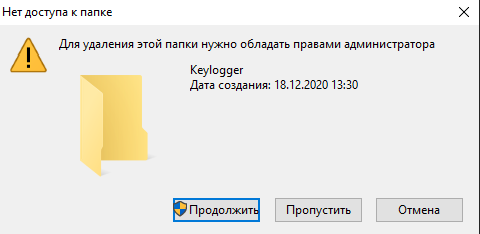
\includegraphics[scale=1]{attachments/delete.png}  
	  \caption{ Ошибка удаления папки }
	  \label{sec:testing:func:deleteerror}
\end{figure}

\begin{table}[htb]
	\caption{Тест-кейс запуска программы без параметров командной строки}
	\label{table:testing:func:test7}
	\centering
	  \begin{tabular}{| >{\raggedright}m{0.4\textwidth} 
					  | >{\raggedright}m{0.3\textwidth} 
					  | >{\raggedright\arraybackslash}m{0.2\textwidth}|}
	  \hline Тест & Ожидаемый результат  & Результат \\
	  \hline \textbf{Запуск без параметров} \\ 1. Запустить программное средство не указывая аргументы командной строки & 1. Сообщение об ошибке & Успех (Рисунок \ref*{sec:testing:func:runerr})\\
	  \hline
	  \end{tabular}
\end{table}

\begin{figure}[htb]
	\centering
	  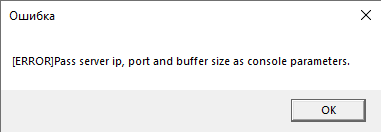
\includegraphics[scale=1]{attachments/runerr.png}  
	  \caption{ Ошибка запуска }
	  \label{sec:testing:func:runerr}
\end{figure}

